\documentclass[tikz,border=10pt]{standalone}
% Scale s = 0.010025 (1 unit = ~100 px), y flipped, origin at px (450,400)
\begin{document}
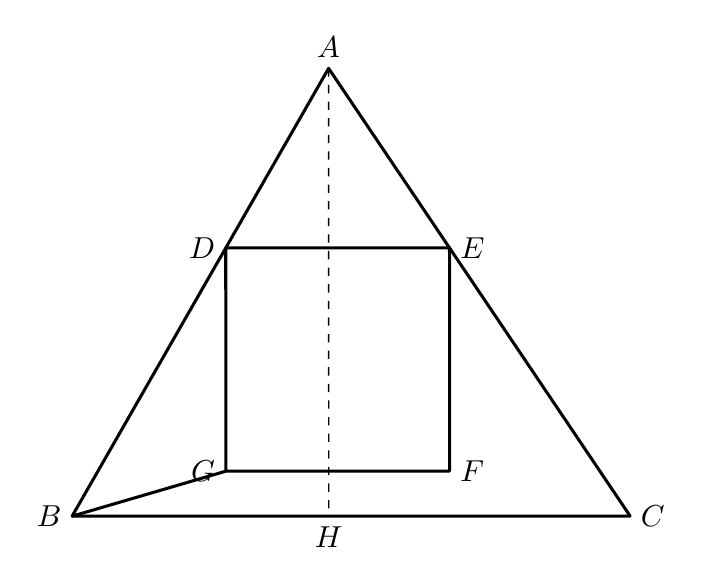
\begin{tikzpicture}[line join=round, line width=1.1pt, font=\fontsize{11}{13.2}\selectfont]
  % Named coordinates (converted from pixels)
  \coordinate (A) at (-0.04452619930858372,2.869061206671248);
  \coordinate (B) at (-3.301639328960162,-2.8182377128639833);
  \coordinate (C) at (3.7844072106650755,-2.8165184065371633);
  \coordinate (D) at (-1.3507251045080375,0.5882857694872079);
  \coordinate (E) at (1.490989586943585,0.5889752622841731);
  \coordinate (F) at (1.491677496643943,-2.2462147650870374);
  \coordinate (G) at (-1.3500371948076795,-2.246904257884003);
  \coordinate (H) at (-0.043146466668140884,-2.8174470960704427);

  % Triangle ABC (solid)
  \draw (A) -- (B) -- (C) -- cycle;

  % Dashed altitude from A to H on BC (thinner stroke)
  \draw[dashed, line width=0.5pt] (A) -- (H);

  % Inner square DEFG (solid)
  \draw (D) -- (E) -- (F) -- (G) -- cycle;

  % Solid segment B to G
  \draw (B) -- (G);

  % Labels
  \node[above] at (A) {$A$};
  \node[left] at (B) {$B$};          % left of B, no vertical offset
  \node[right] at (C) {$C$};         % right of C, no vertical offset
  \node[left] at (D) {$D$};          % left of D, level with vertex (anchor east)
  \node[right] at (E) {$E$};         % right of E, level with vertex (anchor west)
  \node[right] at (F) {$F$};         % right of F, no vertical offset
  \node[left] at (G) {$G$};          % left of G, level with vertex (anchor east)
  \node[below] at (H) {$H$};
\end{tikzpicture}
\end{document}
% GEOAGENT_REPAIR_V1 c18a466396f54661 90be1f9a0a75633230d52fa2f17971aede6041a4030a4f357c6b27a7c3068399